% --------------------------------------------------------------------------- %
% Poster for the ECCS 2011 Conference about Elementary Dynamic Networks.      %
% --------------------------------------------------------------------------- %
% Created with Brian Amberg's LaTeX Poster Template. Please refer for the     %
% attached README.md file for the details how to compile with `pdflatex`.     %
% --------------------------------------------------------------------------- %
% $LastChangedDate:: 2011-09-11 10:57:12 +0200 (V, 11 szept. 2011)          $ %
% $LastChangedRevision:: 128                                                $ %
% $LastChangedBy:: rlegendi                                                 $ %
% $Id:: poster.tex 128 2011-09-11 08:57:12Z rlegendi                        $ %
% --------------------------------------------------------------------------- %
\documentclass[a0paper,portrait]{baposter}

\usepackage{relsize}		% For \smaller
\usepackage{url}			% For \url
% \usepackage{epstopdf}	% Included EPS files automatically converted to PDF to include with pdflatex

%%% Global Settings %%%%%%%%%%%%%%%%%%%%%%%%%%%%%%%%%%%%%%%%%%%%%%%%%%%%%%%%%%%

\graphicspath{{figures/}}	% Root directory of the pictures
% \tracingstats=2			% Enabled LaTeX logging with conditionals

%%% Color Definitions %%%%%%%%%%%%%%%%%%%%%%%%%%%%%%%%%%%%%%%%%%%%%%%%%%%%%%%%%

\definecolor{bordercol}{RGB}{40,40,40}
\definecolor{headercol1}{RGB}{186,215,230}
\definecolor{headercol2}{RGB}{80,180,80}
\definecolor{headerfontcol}{RGB}{0,0,0}
\definecolor{boxcolor}{RGB}{186,215,230}

%%%%%%%%%%%%%%%%%%%%%%%%%%%%%%%%%%%%%%%%%%%%%%%%%%%%%%%%%%%%%%%%%%%%%%%%%%%%%%%%
%%% Utility functions %%%%%%%%%%%%%%%%%%%%%%%%%%%%%%%%%%%%%%%%%%%%%%%%%%%%%%%%%%

%%% Save space in lists. Use this after the opening of the list %%%%%%%%%%%%%%%%
\newcommand{\compresslist}{
  \setlength{\itemsep}{1pt}
  \setlength{\parskip}{0pt}
  \setlength{\parsep}{0pt}
}

%%%%%%%%%%%%%%%%%%%%%%%%%%%%%%%%%%%%%%%%%%%%%%%%%%%%%%%%%%%%%%%%%%%%%%%%%%%%%%%
%%% Document Start %%%%%%%%%%%%%%%%%%%%%%%%%%%%%%%%%%%%%%%%%%%%%%%%%%%%%%%%%%%%
%%%%%%%%%%%%%%%%%%%%%%%%%%%%%%%%%%%%%%%%%%%%%%%%%%%%%%%%%%%%%%%%%%%%%%%%%%%%%%%

\begin{document}
\typeout{Poster rendering started}

%%% Setting Background Image %%%%%%%%%%%%%%%%%%%%%%%%%%%%%%%%%%%%%%%%%%%%%%%%%%
\background{
  \begin{tikzpicture}[remember picture,overlay]%
	\draw (current page.north west)+(-2em,2em) node[anchor=north west]
	{
\includegraphics[height=1.1\textheight]{background}};
  \end{tikzpicture}
}

%%% General Poster Settings %%%%%%%%%%%%%%%%%%%%%%%%%%%%%%%%%%%%%%%%%%%%%%%%%%%
%%%%%% Eye Catcher, Title, Authors and University Images %%%%%%%%%%%%%%%%%%%%%%
\begin{poster}{
	grid=false,
	% Option is left on true though the eyecatcher is not used. The reason is
	% that we have a bit nicer looking title and author formatting in the headercol
	% this way
	% eyecatcher=false,
	borderColor=bordercol,
	headerColorOne=headercol1,
	headerColorTwo=headercol2,
	headerFontColor=headerfontcol,
	% Only simple background color used, no shading, so boxColorTwo isn't necessary
	boxColorOne=boxcolor,
	headershape=roundedright,
	headerfont=\Large\sf\bf,
	textborder=rectangle,
	background=user,
	headerborder=open,
	boxshade=plain,
  }
  %%% Eye Cacther %%%%%%%%%%%%%%%%%%%%%%%%%%%%%%%%%%%%%%%%%%%%%%%%%%%%%%%%%%%%%%%
  {
	Eye Catcher, empty if option eyecatcher=false - unused
  }
  %%% Title %%%%%%%%%%%%%%%%%%%%%%%%%%%%%%%%%%%%%%%%%%%%%%%%%%%%%%%%%%%%%%%%%%%%%
  {\sf\bf
	Practical Memory Reclaim with Cgroups and Ballooning
  }
  %%% Authors %%%%%%%%%%%%%%%%%%%%%%%%%%%%%%%%%%%%%%%%%%%%%%%%%%%%%%%%%%%%%%%%%%%
  {
	\vspace{1em} David \textsc{Baldassin}, Guillaume \textsc{Urvoy-Keller}, Dino \textsc{Lopez Pacheco} \\
	{\smaller baldassin@i3s.unice.fr, guillaume.urvoy-keller@univ-cotedazur.fr, dino.lopez@univ-cotedazur.fr}
  }
  %%% Logo %%%%%%%%%%%%%%%%%%%%%%%%%%%%%%%%%%%%%%%%%%%%%%%%%%%%%%%%%%%%%%%%%%%%%%
  {
	% The logos are compressed a bit into a simple box to make them smaller on the result
	% (Wasn't able to find any bigger of them.)
	\setlength\fboxsep{0pt}
	\setlength\fboxrule{0.5pt}
	\fbox{
	  \begin{minipage}{14em}
		
\includegraphics[width=14em,height=8em]{logo_trans}
	  \end{minipage}
	}
  }

  \headerbox{Problem}{name=problem,column=0,row=0}{

	\begin{itemize}
	  \item In datacenters, memory become the limiting factor when adding new VMs
	  \item VMs are usually over-allocated
	  \item Guest OS only use a subset of the memory allocated for the VM
	  \item Hypervisor does not track memory liberation by the Guest
	\end{itemize}

	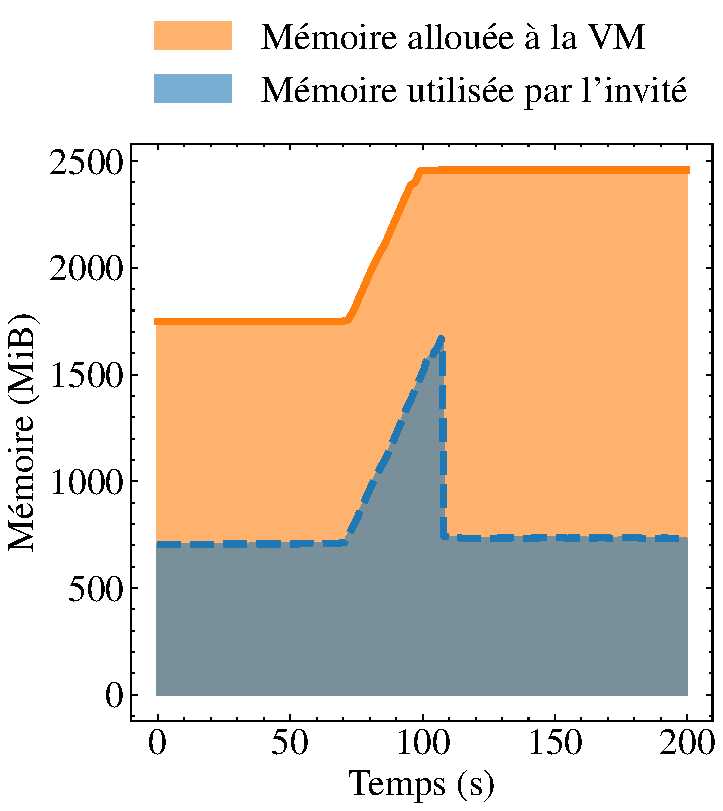
\includegraphics[width=\linewidth]{memory_area_plot}
  }

  \headerbox{Basic Concepts}{name=definitions,column=0,below=problem}{
	\begin{itemize}
	  \item \textbf{cgroups} : Linux kernel feature to monitor process resources.
	  \item \textbf{ballooning} : Kernel module within guest OS to inform the hypervisor and reserve free memory page.
	\end{itemize}
  }

  \headerbox{Testbed}{name=testbed,column=0,below=definitions}{
	  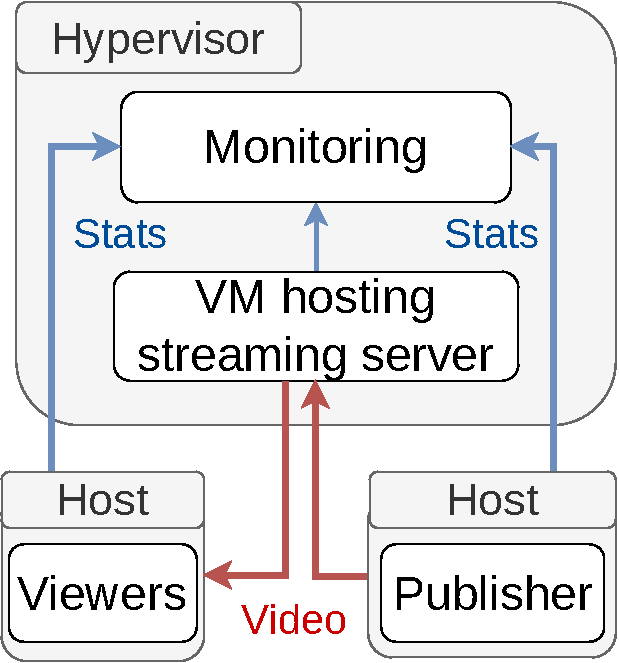
\includegraphics[width=\linewidth]{testbed}
  }

  % \headerbox{Models}{name=models,column=0,below=definitions}{
  % 	\textbf{ER1} $G_0$ is a random graph. Add each non-existing edge with $p_A$, delete each existing edge with $p_D$ probability. \\
  % 	\textbf{ER2} $G_0$ is a random graph. Add $k_A$ uniformly selected random new edges and delete $k_D$ existing edges. \\
  % 	\textbf{ER3} $G_0$ is a random graph. Rewire $k_{RW}$ edges. \\
  % 	\textbf{SPA} (\emph{Snapshot preferential}) $G_0$ is a scale free network. Add $k_A$ edges from a random node with preferential attachment based on the snapshot network. Delete $k_D$ existing edges. \\
  % 	\textbf{CPA} (\emph{Cumulative preferential}) $G_0$ is a scale free network. Add $k_A$ edges from a random node with preferential attachment based on the cumulative network. Delete $k_D$ existing edges.
  % }

  \headerbox{References}{name=references,column=0,below=testbed}{
	\smaller													% Make the whole text smaller
	\vspace{-0.4em} 										% Save some space at the beginning
	\bibliographystyle{plain}							% Use plain style
	\renewcommand{\section}[2]{\vskip 0.05em}		% Omit "References" title
	\begin{thebibliography}{1}							% Simple bibliography with widest label of 1
	  \itemsep=-0.01em										% Save space between the separation
	  \setlength{\baselineskip}{0.4em}					% Save space with longer lines
	  % \bibitem{prevWork1} Laszlo Gulyas, Richard Legendi: \emph{Effects of Sample Duration on Network Statistics in Elementary Models of Dynamic Networks}, International Conference on Computational Science, Singapore (2011)
	  % \bibitem{prevWork2} Laszlo Gulyas, Susan Khor, Richard Legendi and George Kampis \emph{Cumulative Properties of Elementary Dynamic Networks}, The International Sunbelt Social Network Conference XXXI (2011)
	  % \bibitem{gulya-kampis1} Gulyas, Laszlo et al.: \emph{Betweenness Centrality Dynamics in Networks of Changing Density}. Presented at the 19th International Symposium on Mathematical Theory of Networks and Systems (MTNS 2010)
	\end{thebibliography}
  }

  % \headerbox{Acknowledgements}{name=acknowledgements,column=0,below=references, above=bottom}{
  % 	\smaller						% Make the whole text smaller
  % 	\vspace{-0.4em}			% Save some space at the beginning
  % 	This research was partially supported by the Hungarian Government (KMOP-1.1.2-08/1-2008-0002 ) and the European Union's Seventh Framework Programme: DynaNets, FET-Open project no. FET-233847 (\url{http://www.dynanets.org}). The supports are gratefully acknowledged.
  % }

  \headerbox{Heuritics based on cgroups}{name=heuristics-cgroups,column=1,row=0}{
	% \begin{minipage}{\linewidth}
	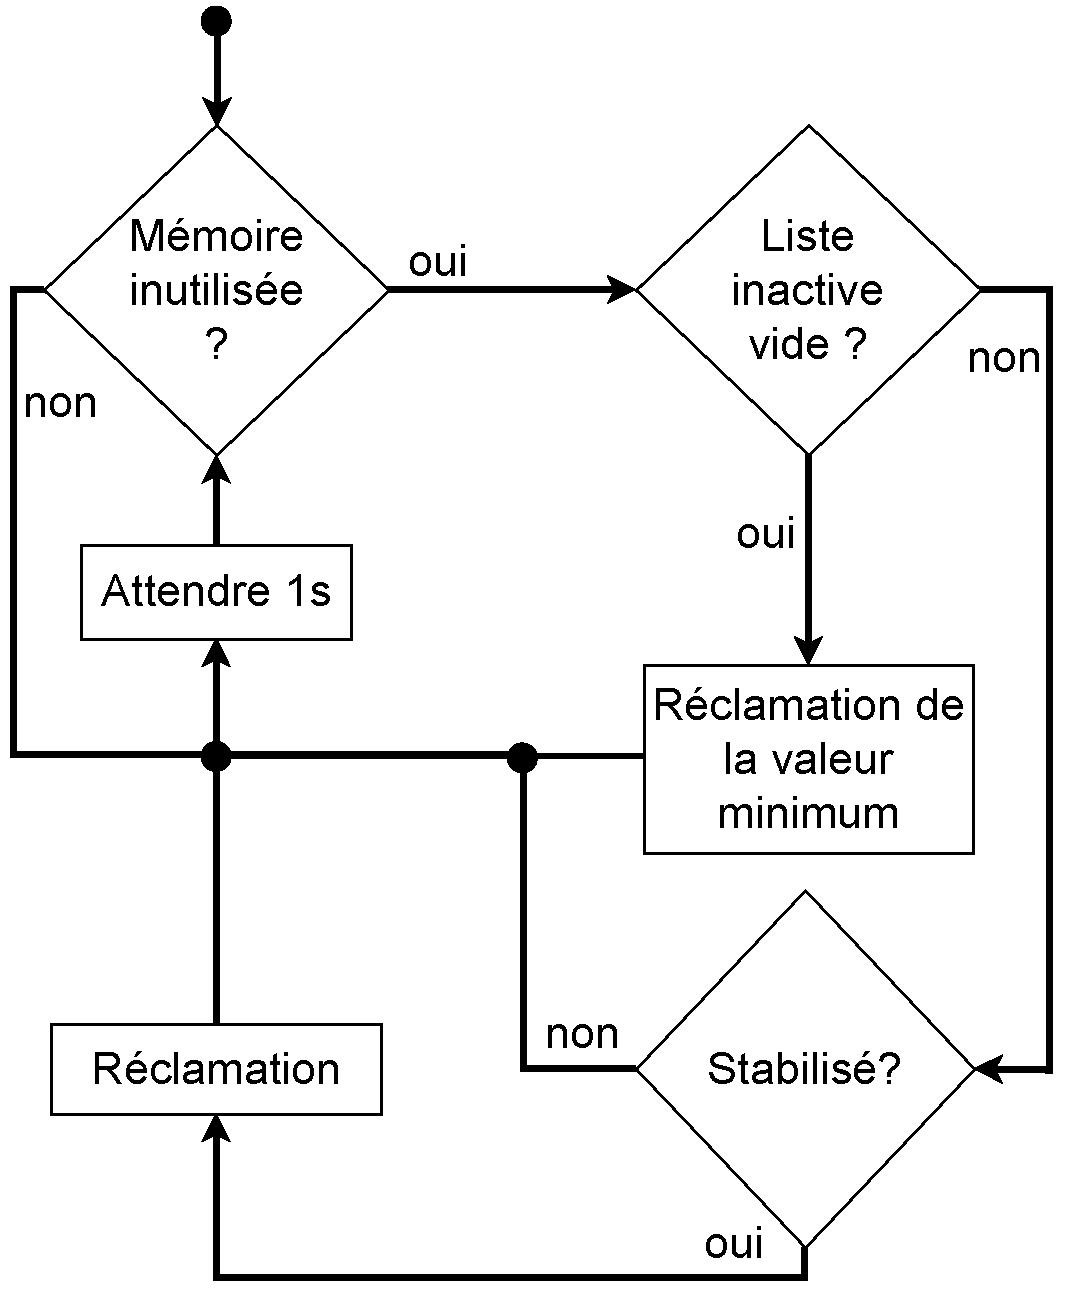
\includegraphics[width=\linewidth]{heuristic_reclaim}
	% 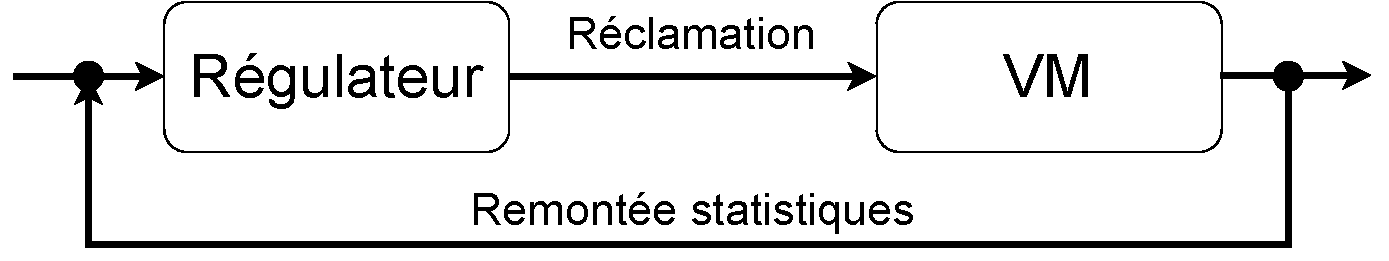
\includegraphics[width=\linewidth]{retroaction}
	% \end{minipage}
  }

  \headerbox{Heuritics based on ballooning}{name=heuristics-ballooning,column=2,row=0}{
	% \begin{minipage}{\linewidth}
	% 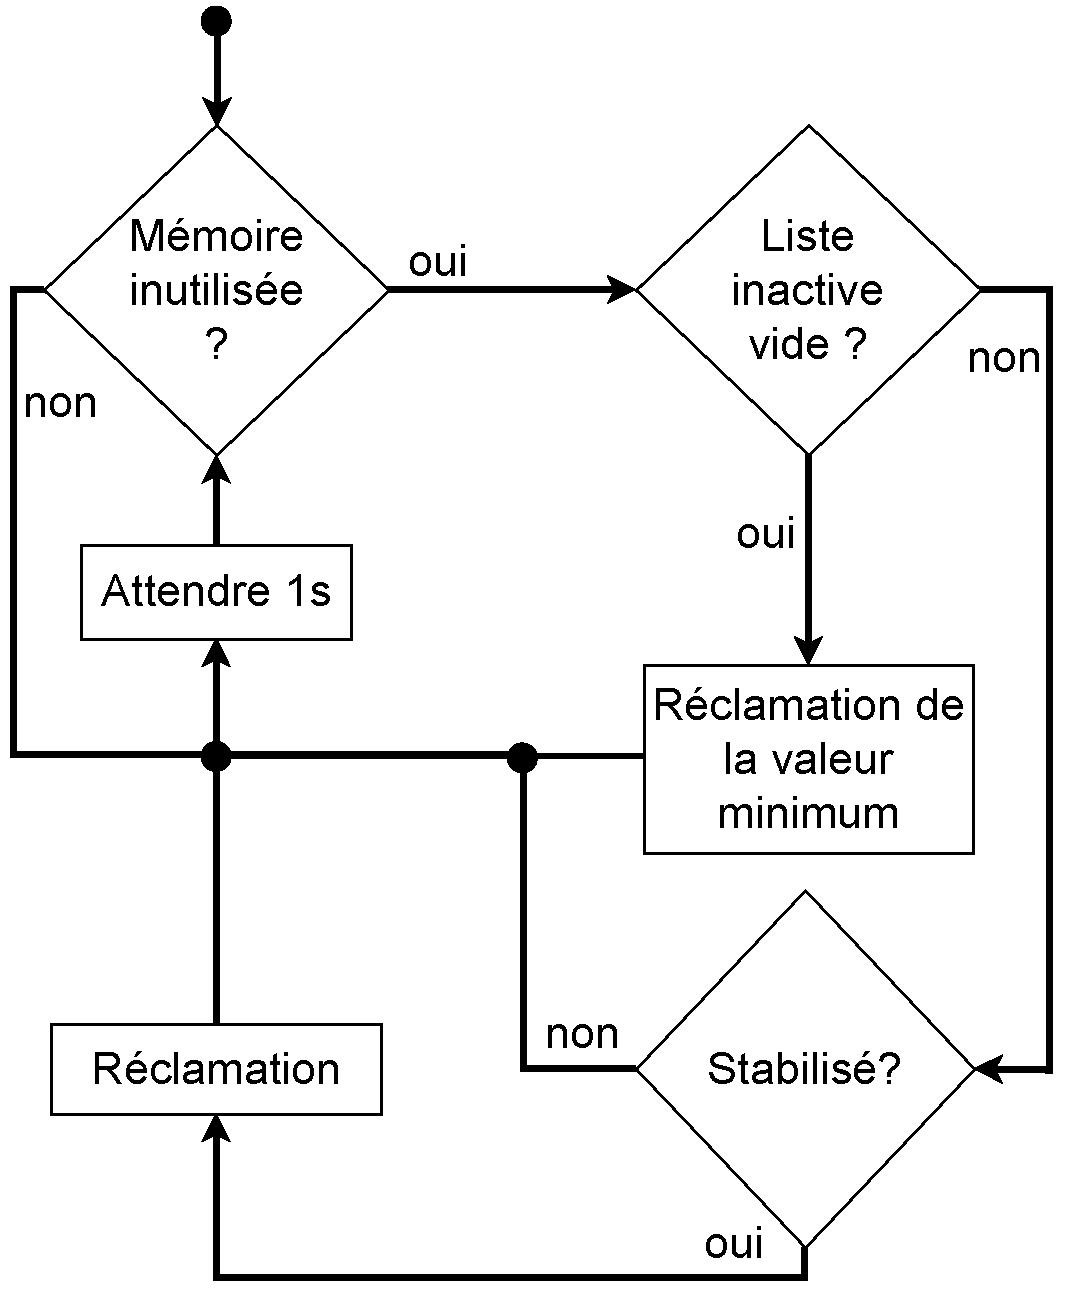
\includegraphics[width=\linewidth]{heuristic_reclaim}
	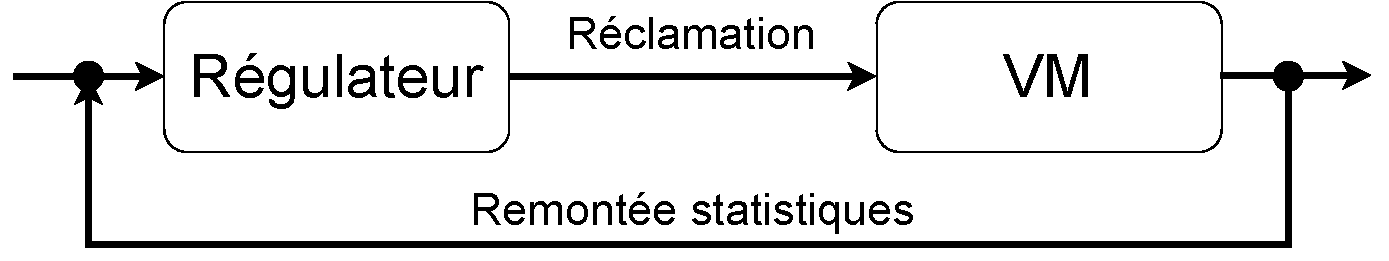
\includegraphics[width=\linewidth]{retroaction}

    \begin{itemize}
      \item Based on PID regulation
      \item Safety margin of 200~MiB
      \item + Reactive
      \item - CPU consumption
    \end{itemize}

	% \end{minipage}
  }

  \headerbox{Results with cgroups}{name=results-cgroups,span=1,column=1,below=heuristics-cgroups}{
	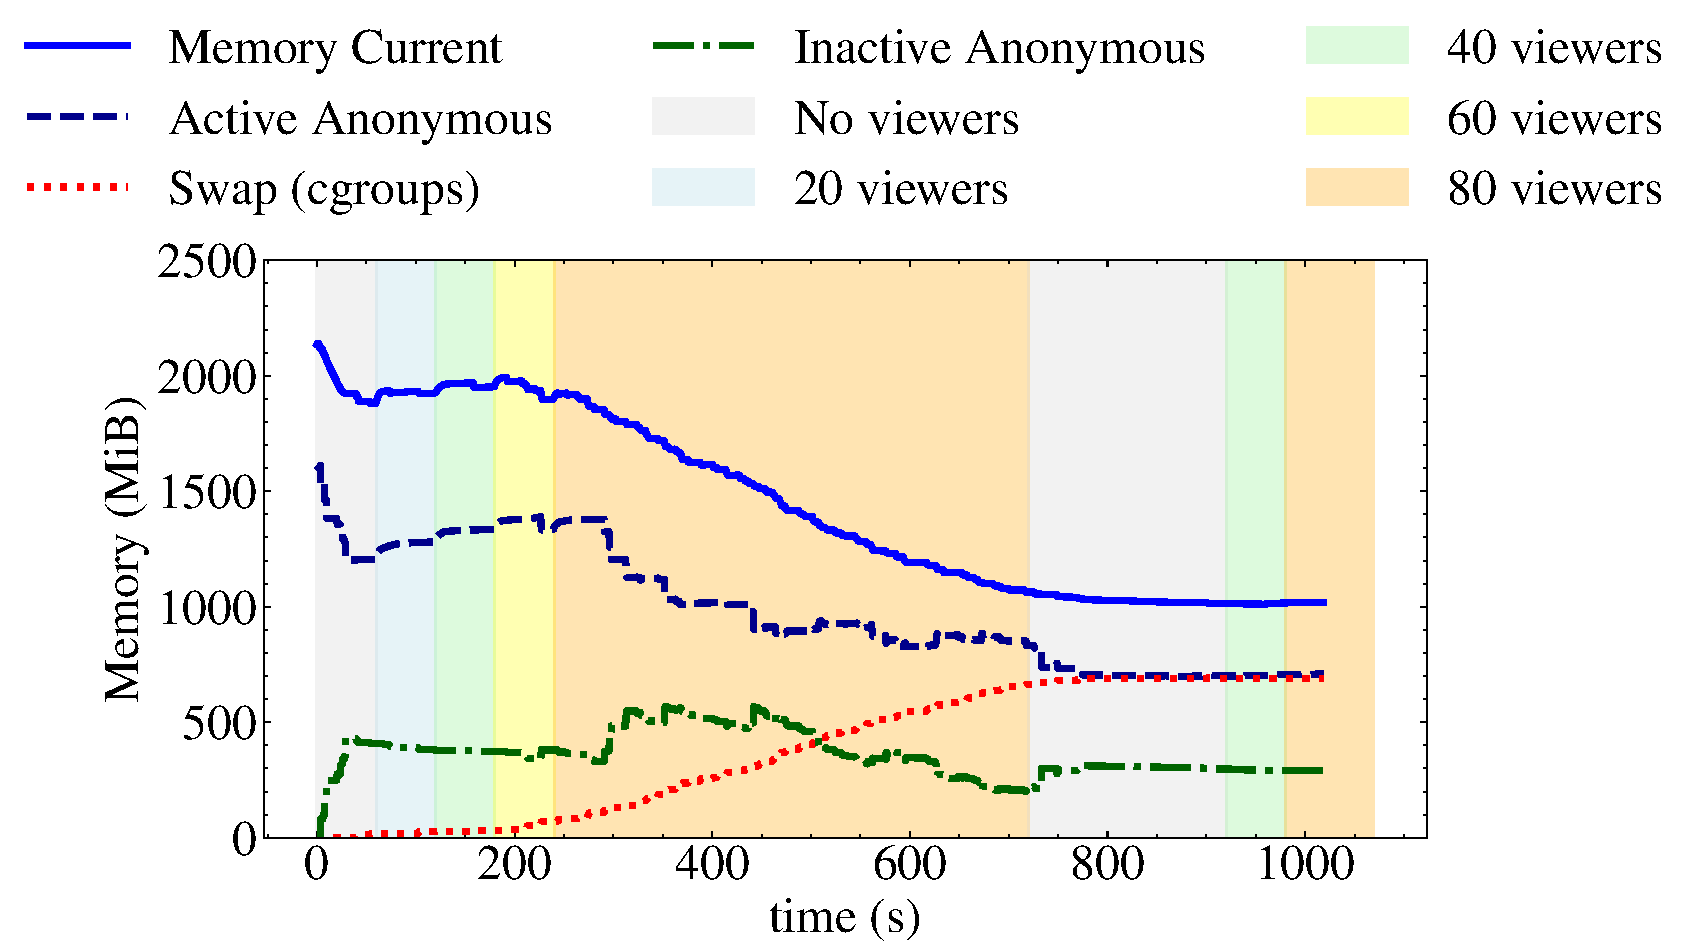
\includegraphics[width=\linewidth]{res_cgroups}
  }

  \headerbox{Results with ballooing}{name=results-ballooning,span=1,column=2,below=heuristics-ballooning}{
	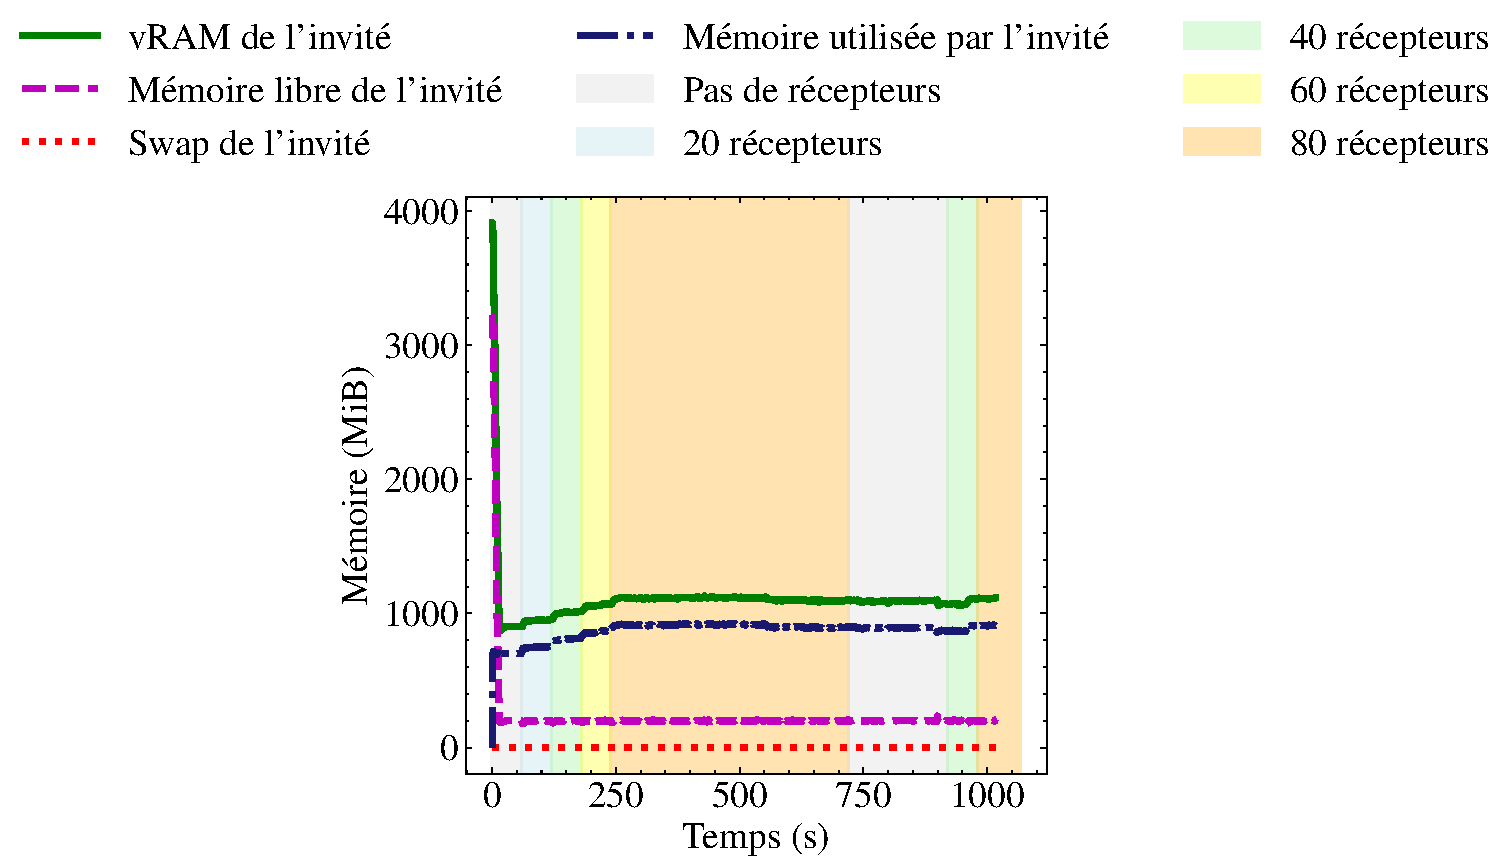
\includegraphics[width=\linewidth]{res_balloon}
  }

  \headerbox{Quality of Service (publishing bitrate) is not affected}{name=qos,span=2,column=1,below=results-cgroups}{
	  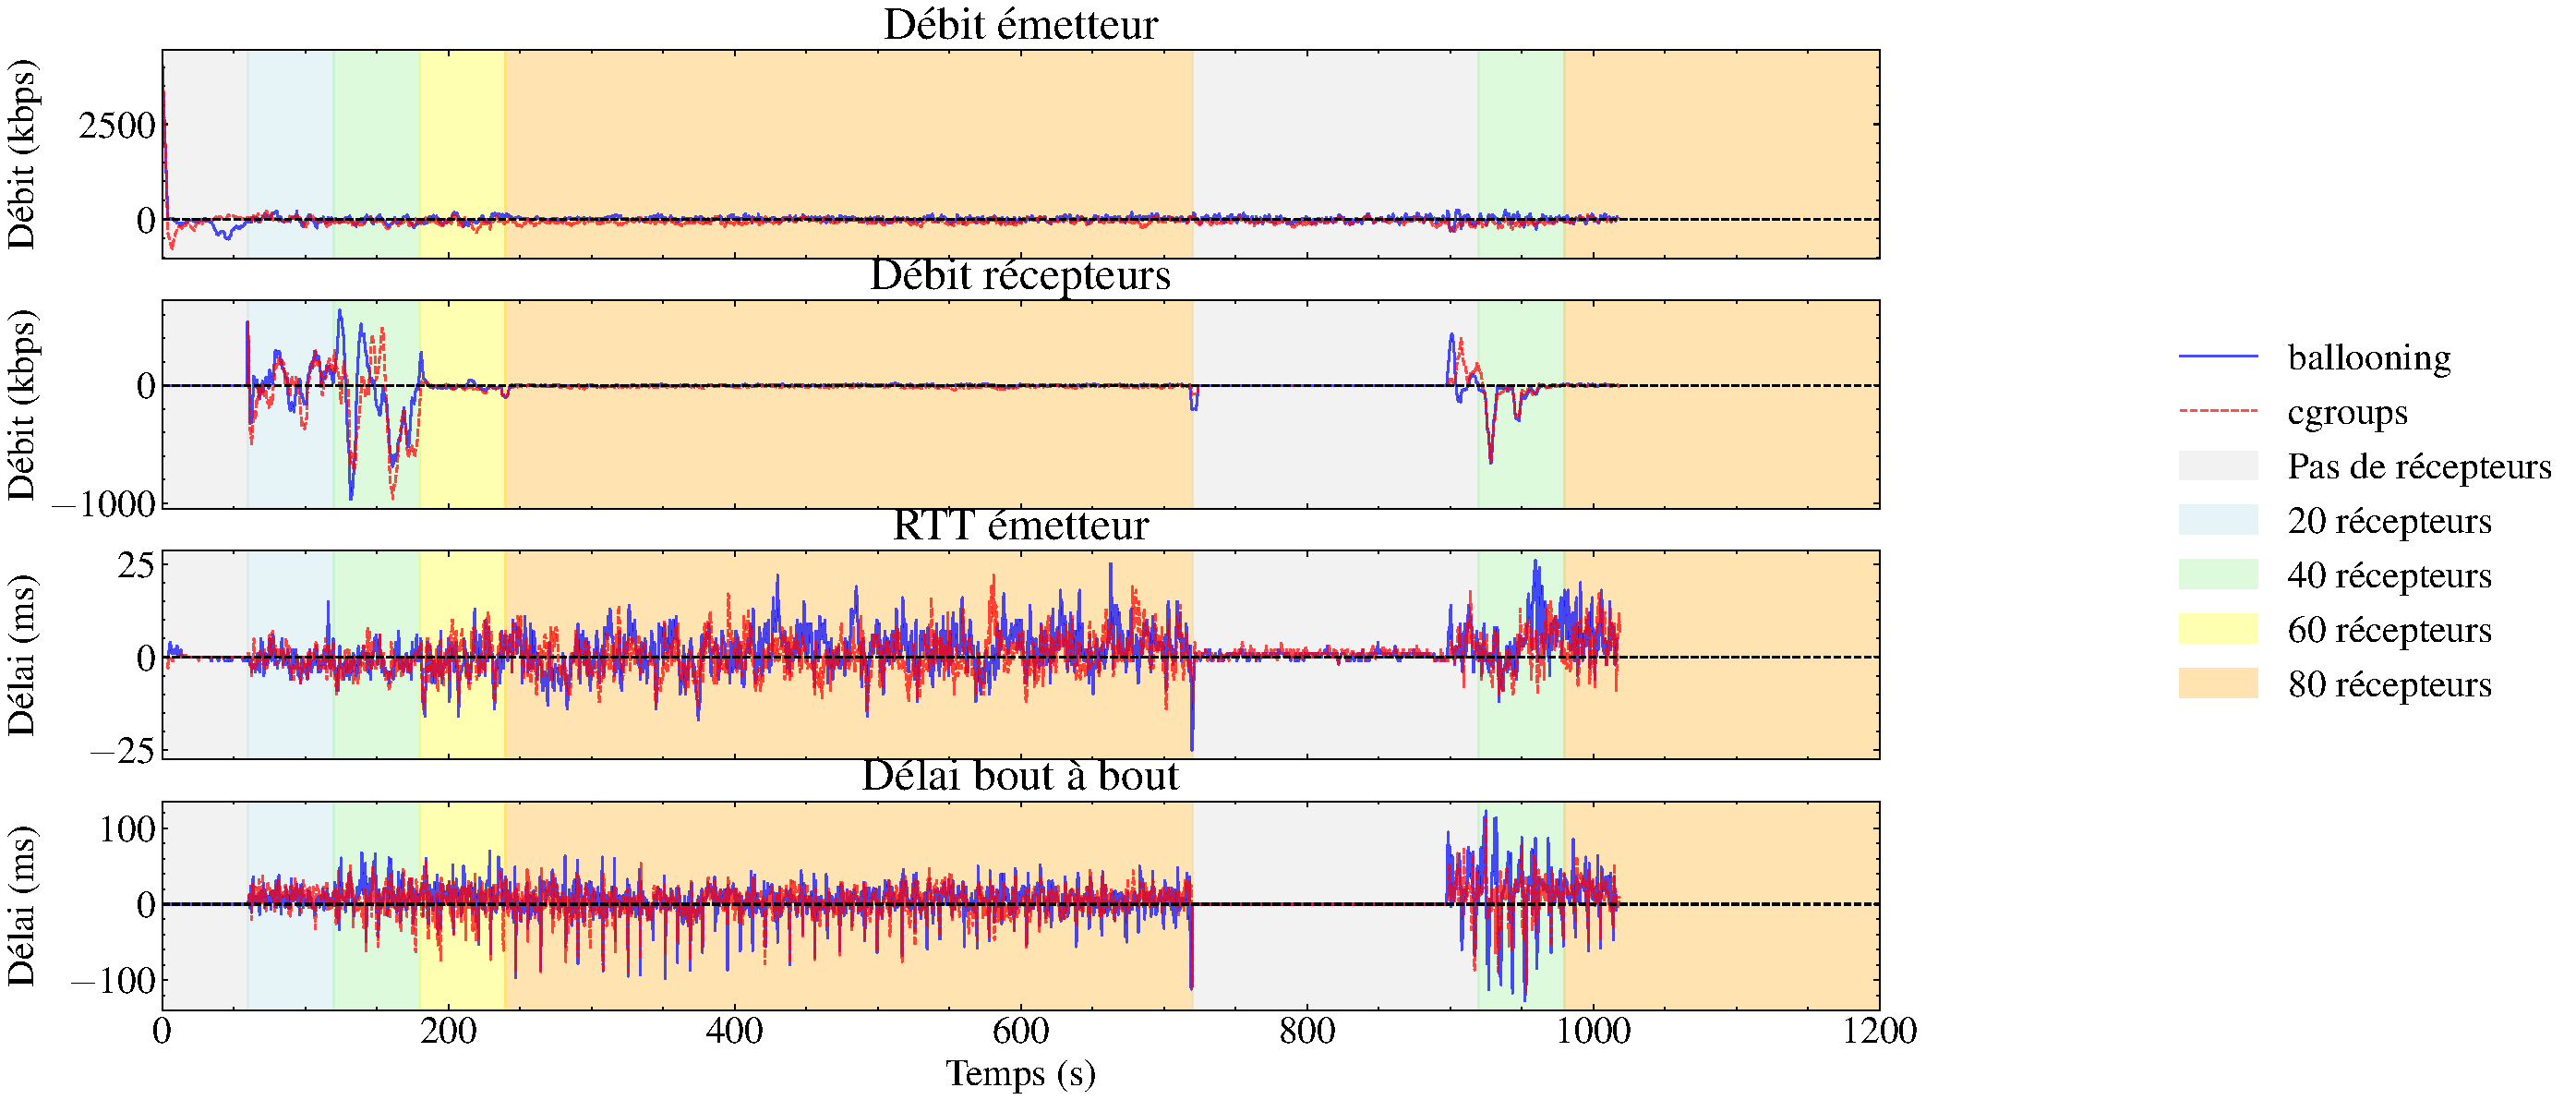
\includegraphics[width=\linewidth]{delta}
  }

  \headerbox{Additional VMs using our heuristics}{name=vm-load,span=2,column=1,below=qos,above=bottom}{
	\begin{minipage}[h!]{\linewidth}
      \begin{minipage}[h!]{0.3\linewidth}
        \begin{itemize}
          \item 60\% additional VMs with cgroups
          \item 13\% additional VMs with ballooning
        \end{itemize}
      \end{minipage}
      \begin{minipage}{0.6\linewidth}
        \begin{flushright}
          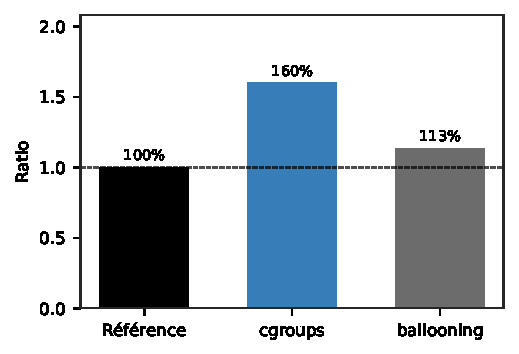
\includegraphics[width=0.9\linewidth]{barplot_vms}
        \end{flushright}
      \end{minipage}
	\end{minipage}
  }

  % \headerbox{Autres}{name=Autre,column=2,row=0}{
  %   % \begin{minipage}{\linewidth}
  %   %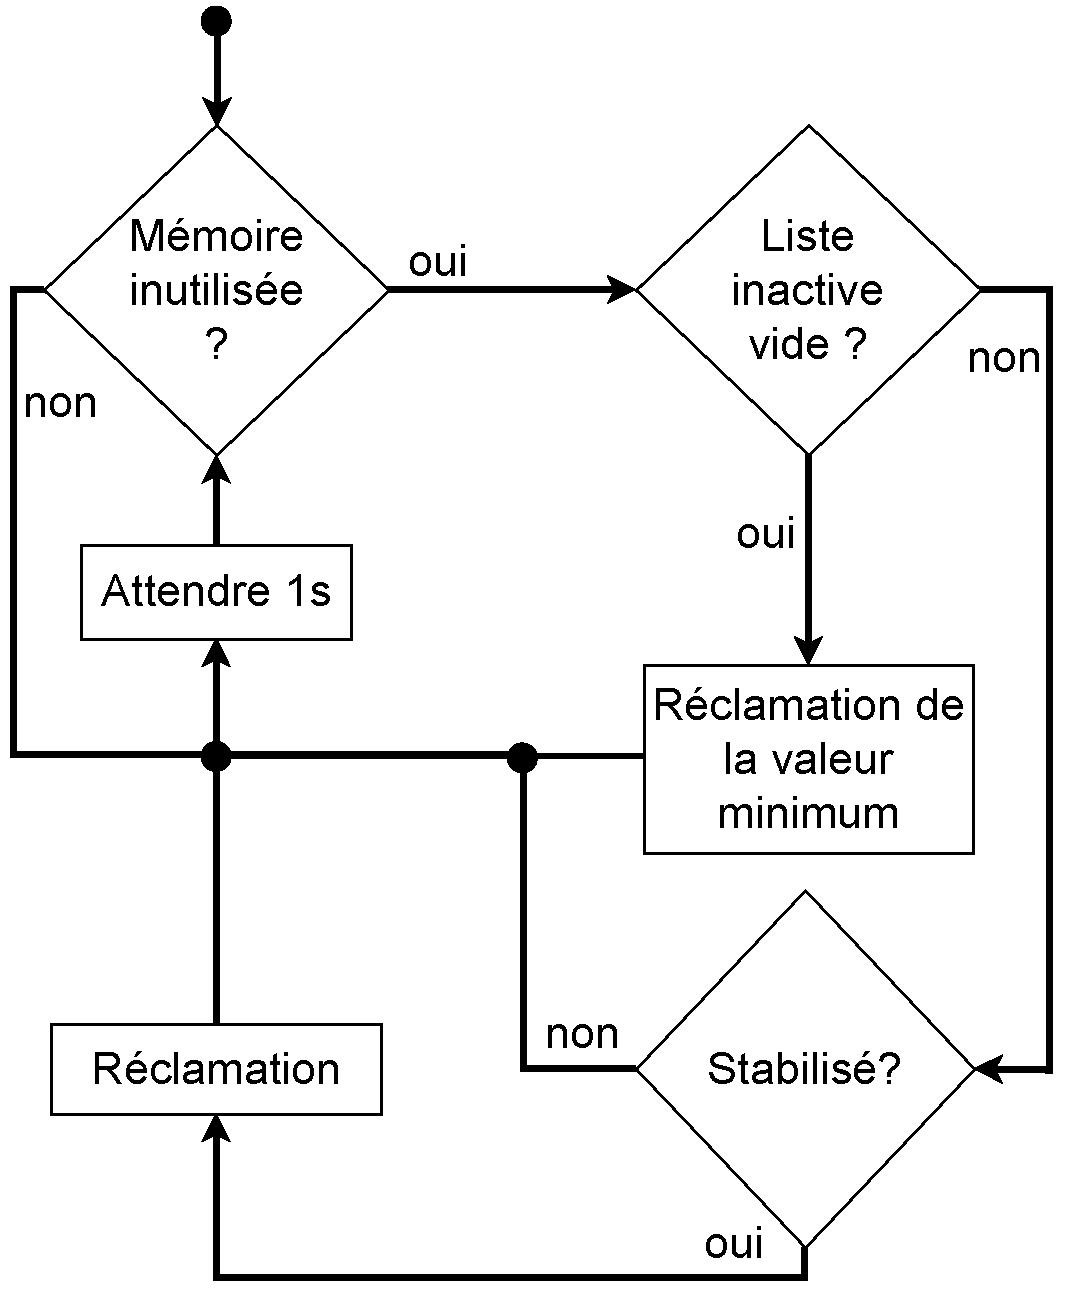
\includegraphics[width=0.5\linewidth]{heuristic_reclaim}
  %   % 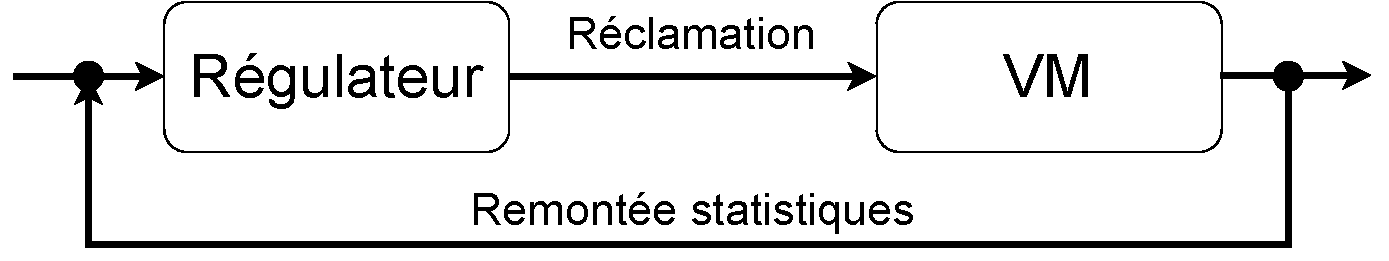
\includegraphics[width=0.5\linewidth]{retroaction}
  %   % \end{minipage}
  % }

\end{poster}
\end{document}
